\documentclass[a4paper]{scrartcl}

\usepackage[utf8]{inputenc}
\usepackage{graphicx}
\usepackage[table]{xcolor}
\usepackage{lscape}
\usepackage{hyperref}
\usepackage{float}

\newcolumntype{g}{>{\columncolor{lightgray}}l}

\title{Design for the practical task of the course CBSE}
\author{Stefan Beyer, Ronny Marx, Manuel Oddoy, Lars Schütze \\
	\{firstname.lastname\}@mailbox.tu-dresden.de}
\date{\today}

\begin{document}

\maketitle
\pagebreak

\tableofcontents
\pagebreak

\section{Requirements}
\subsection{Business concept model}

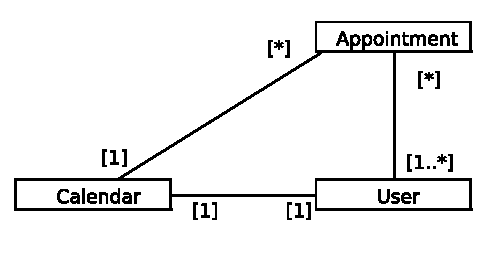
\includegraphics{pictures/BusinessConceptModel}

\subsection{Use case model}
\subsubsection{Register user}

\begin{tabular}{|g|l|}
	\hline Name      & Register user                                 \\ 
	\hline Initiator & User                                          \\ 
	\hline Goal      & Register with the system to create an account \\ 
	\hline
\end{tabular}

\paragraph{Main success scenario:}
\begin{enumerate}
	\item User click register.
	\item User enters his name, email address and password.
	\item User submits data.
	\item System checks user details.
	\item System registers the user.
\end{enumerate}

\paragraph{Extensions:}
\begin{enumerate}
	\item[3] User did not fill all forms.
		\begin{enumerate}
			\item System prompts to fill all forms.
		\end{enumerate}
	\item[4] System detects a user already existing with given email.
		\begin{enumerate}
			\item Fail.
		\end{enumerate}
\end{enumerate}


\paragraph{Variations:}
\begin{itemize}
	\item At every stage the user may abort.
\end{itemize}

\subsubsection{Login}

\begin{tabular}{|g|l|}
	\hline Name      & Login                                         \\ 
	\hline Initiator & User                                          \\ 
	\hline Goal      & Identify user and grant user access to system \\ 
	\hline
\end{tabular}

\paragraph{Main success scenario:}
\begin{enumerate}
	\item user enters email
	\item user enters password
	\item user submits data
	\item system checks email/password
	\item system grants access
\end{enumerate}

\paragraph{Extensions:}
\begin{enumerate}
	\item[4] user/pw do not match or user does not exist
		\begin{enumerate}
			\item display error message: "username or password incorrect!"
			\item resume 1.
		\end{enumerate}
\end{enumerate}


\paragraph{Variations:}
\begin{itemize}
	\item	user may abort in steps 1 to 3
\end{itemize}

\subsubsection{Create appointment}

\begin{tabular}{|g|l|}
	\hline Name      & Create appointment                 \\ 
	\hline Initiator & User                               \\ 
	\hline Goal      & The user creates a new appointment \\ 
	\hline
\end{tabular}

\paragraph{Main success scenario:}
\begin{enumerate}
	\item User enters the title of the appointment
	\item User enters the begin date (including time) and the end date (including time)
	\item User mark appointment as public or private
	\item User choose an category for the appointment
		(being either free, blocked, protentially blocked or away)
	\item User confirms creation
	\item System checks for conflicts
	\item System creates the appointment
\end{enumerate}

\paragraph{Extensions:}
\begin{enumerate}
	\item[1] User did not enter a title
		\begin{enumerate}
			\item System prints an error message
			\item Resume 1.
		\end{enumerate}
	\item[6] There is a private conflicting appointment
		\begin{enumerate}
			\item System notifies the user that there is a conflicting appointment
			\item Resume 2.
		\end{enumerate}
	\item[6] There is a public conflicting appointment
		\begin{enumerate}
			\item System notifies the user that there is a conflicting appointment
				and provides details about the conflicting appointment
			\item Resume 2.
		\end{enumerate}
\end{enumerate}


\paragraph{Variations:}
\begin{itemize}
	\item At 2 the user may invite other users to the appointment.
	\item At every stage the user may abort.
\end{itemize}

\subsubsection{Show appointments of the day}

\begin{tabular}{|g|l|}
	\hline Name      & Show appointments of the day         \\ 
	\hline Initiator & User                                 \\ 
	\hline Goal      & Show list of appointments for a date \\ 
	\hline
\end{tabular}

\paragraph{Main success scenario:}
\begin{enumerate}
	\item User requests the appointments from the appointment manager. Optionally gives a date.
	\item The appointment manager determines the appointments of the User
	\item The appointment manager selects the appointments of the date
	\item Deliver the appointments to the User 
\end{enumerate}

\paragraph{Extensions:}
\begin{enumerate}
	\item[3] Date not given
		\begin{enumerate}
			\item Determine current date
		\end{enumerate}
\end{enumerate}


\paragraph{Variations:}

\begin{landscape}
\section{Specification}
\subsection{Business type model}
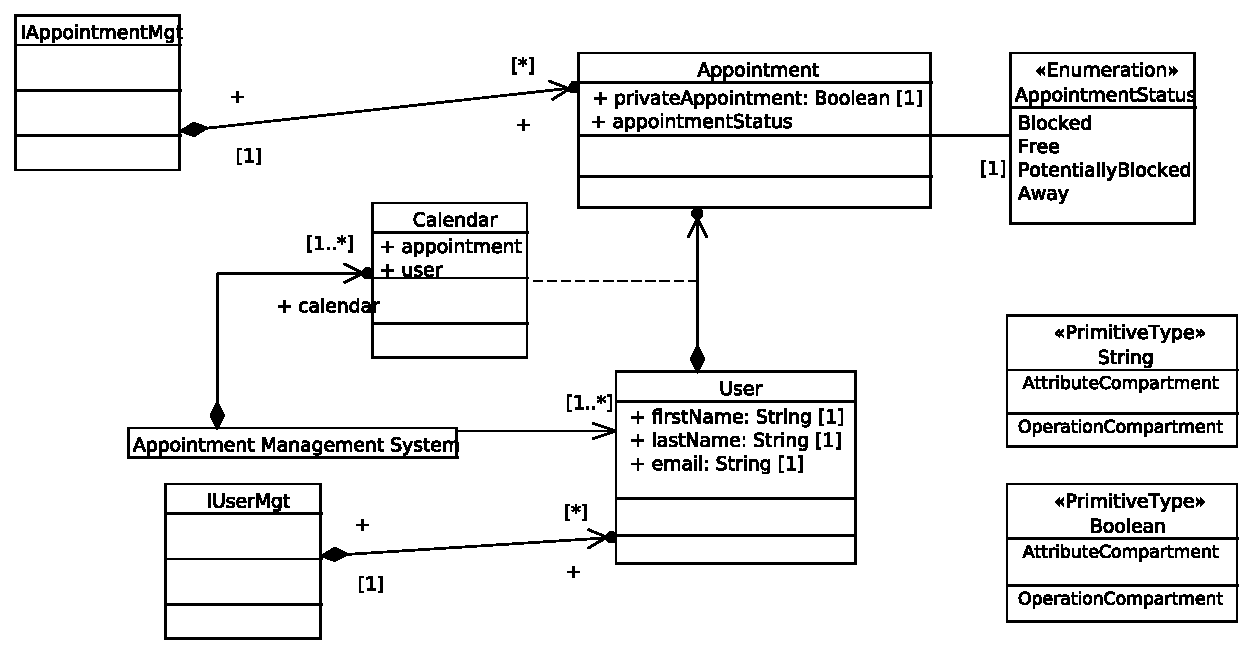
\includegraphics{pictures/BusinessTypeModel}
\end{landscape}

\subsection{Component specifications}

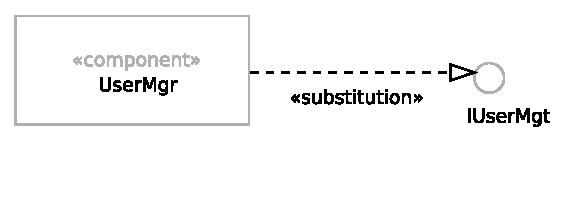
\includegraphics{pictures/UserMgr}

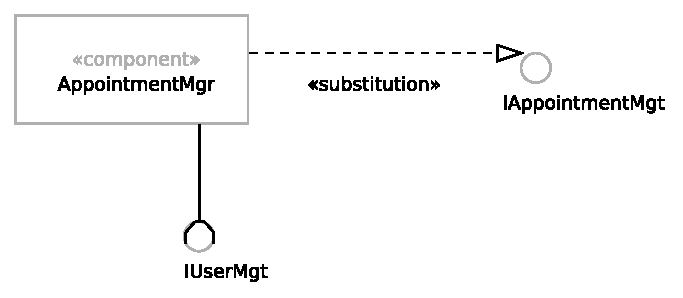
\includegraphics{pictures/AppointmentMgr}

\subsection{Use case map to system interfaces}

\begin{figure}[H]
	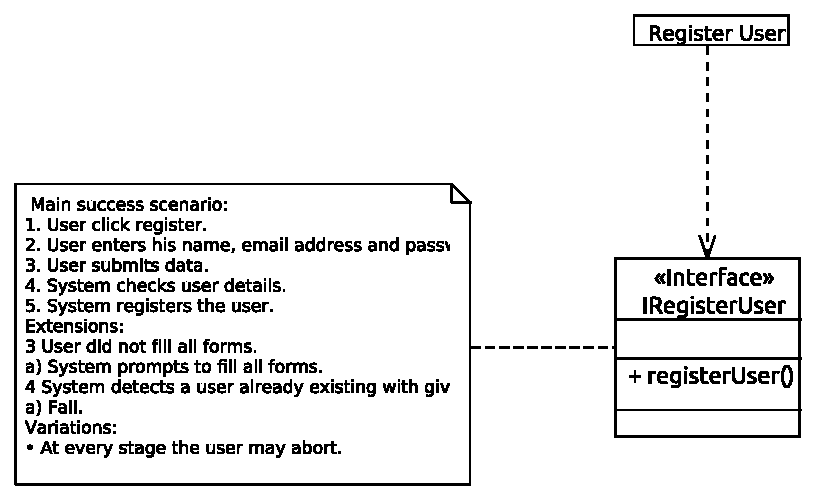
\includegraphics[width=1\textwidth]{pictures/RegisterUser}
	\caption{Register user interface specification}
\end{figure}
\begin{figure}[H]
	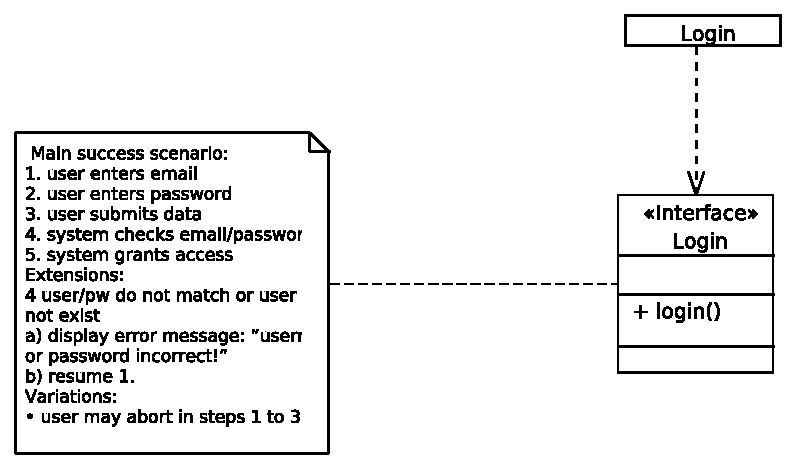
\includegraphics[width=1\textwidth]{pictures/Login}
	\caption{Login interface specification}
\end{figure}
\begin{figure}[H]
	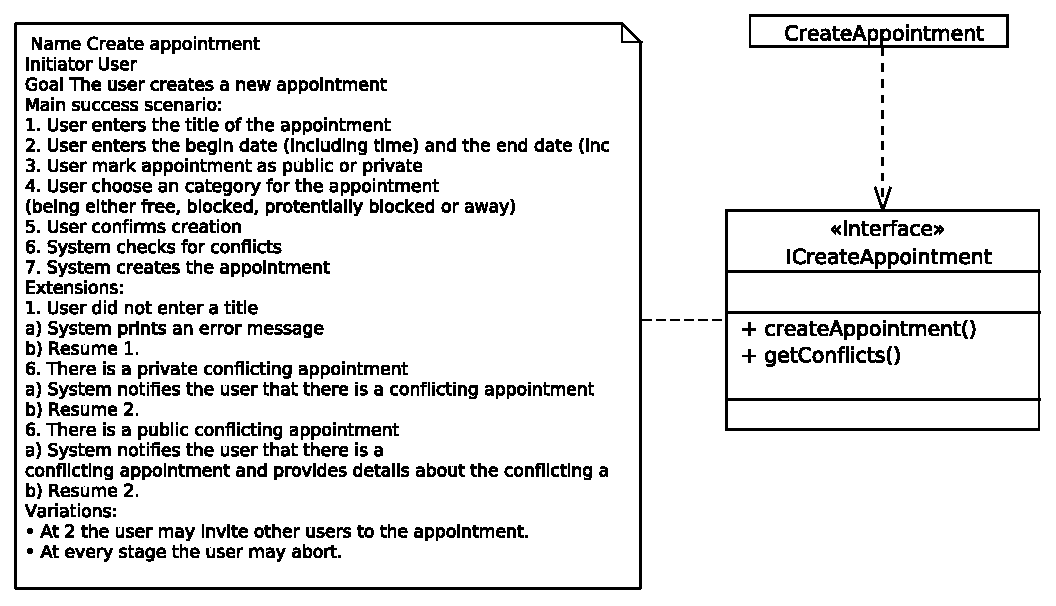
\includegraphics[width=1\textwidth]{pictures/CreateAppointment}
	\caption{Create appointment interface specification}
\end{figure}
\begin{figure}[H]
	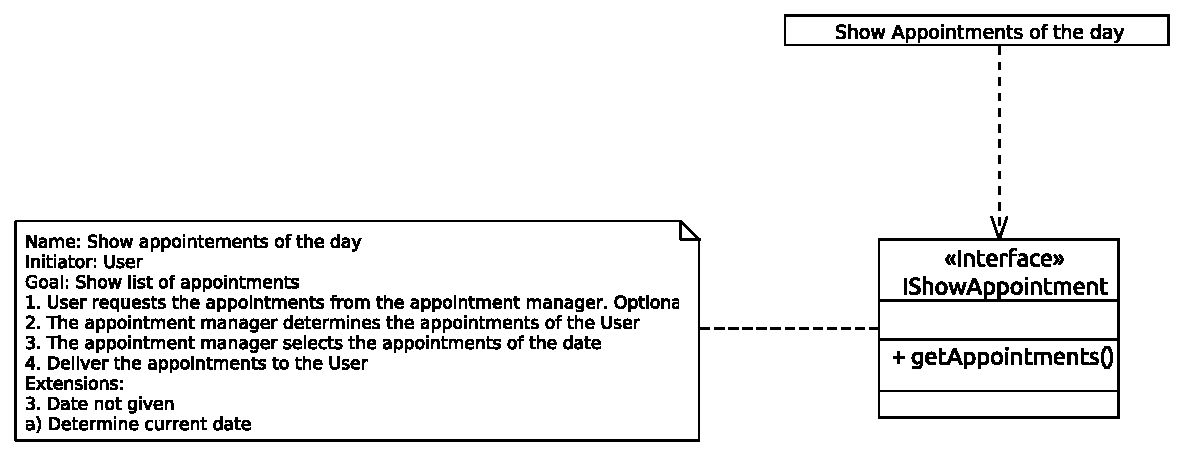
\includegraphics[width=1\textwidth]{pictures/ShowAppointmentsOfTheDay}
	\caption{Show appointments of the day interface specification}
\end{figure}




\subsection{Component architecture}
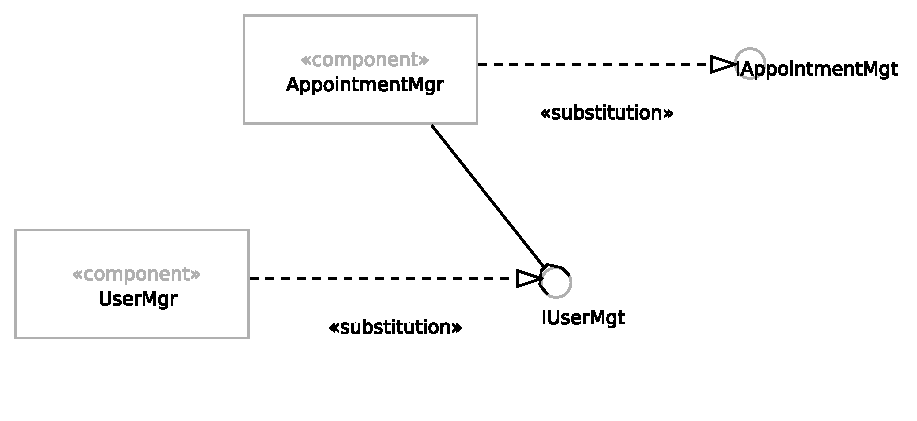
\includegraphics[width=\textwidth]{pictures/ComponentArchitecture}

\subsection{Interface specifications}
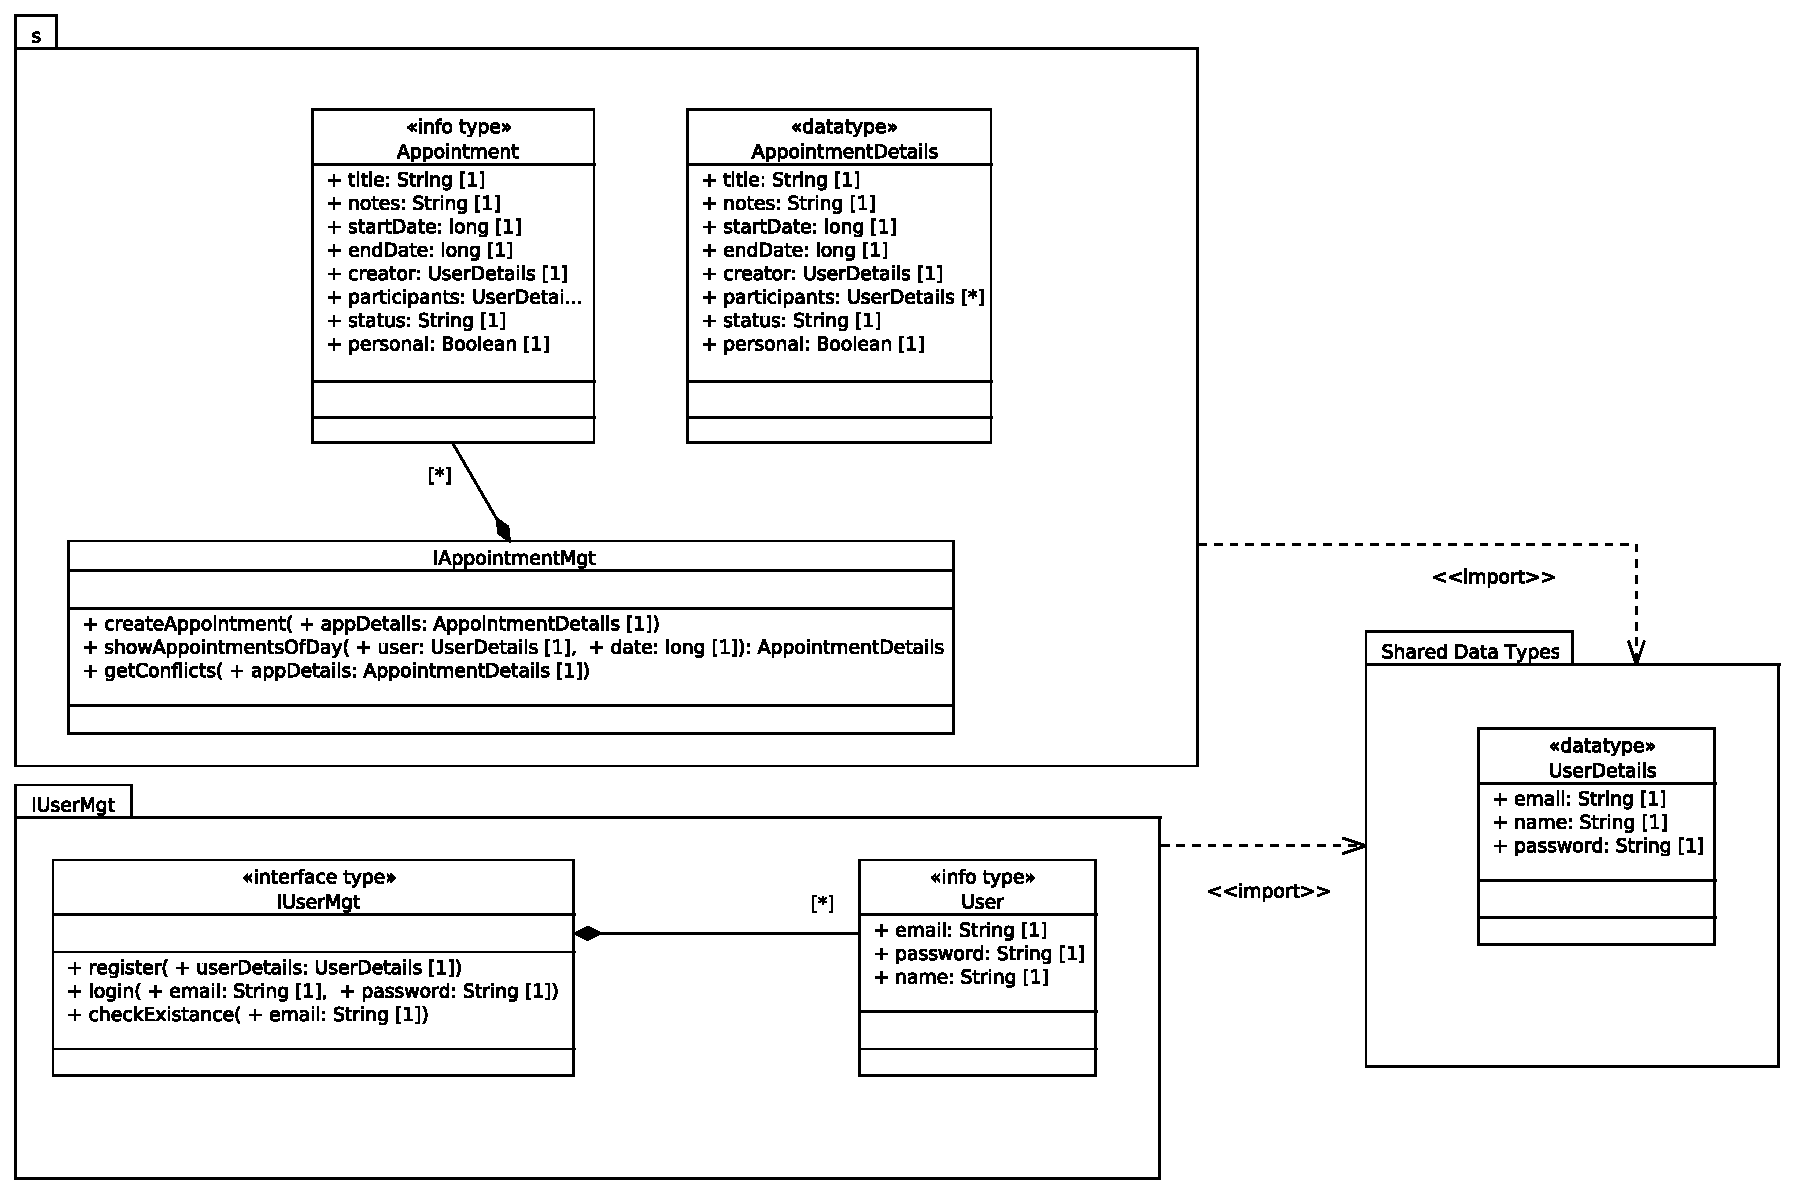
\includegraphics[width=\textwidth]{pictures/InterfaceSpecification}
%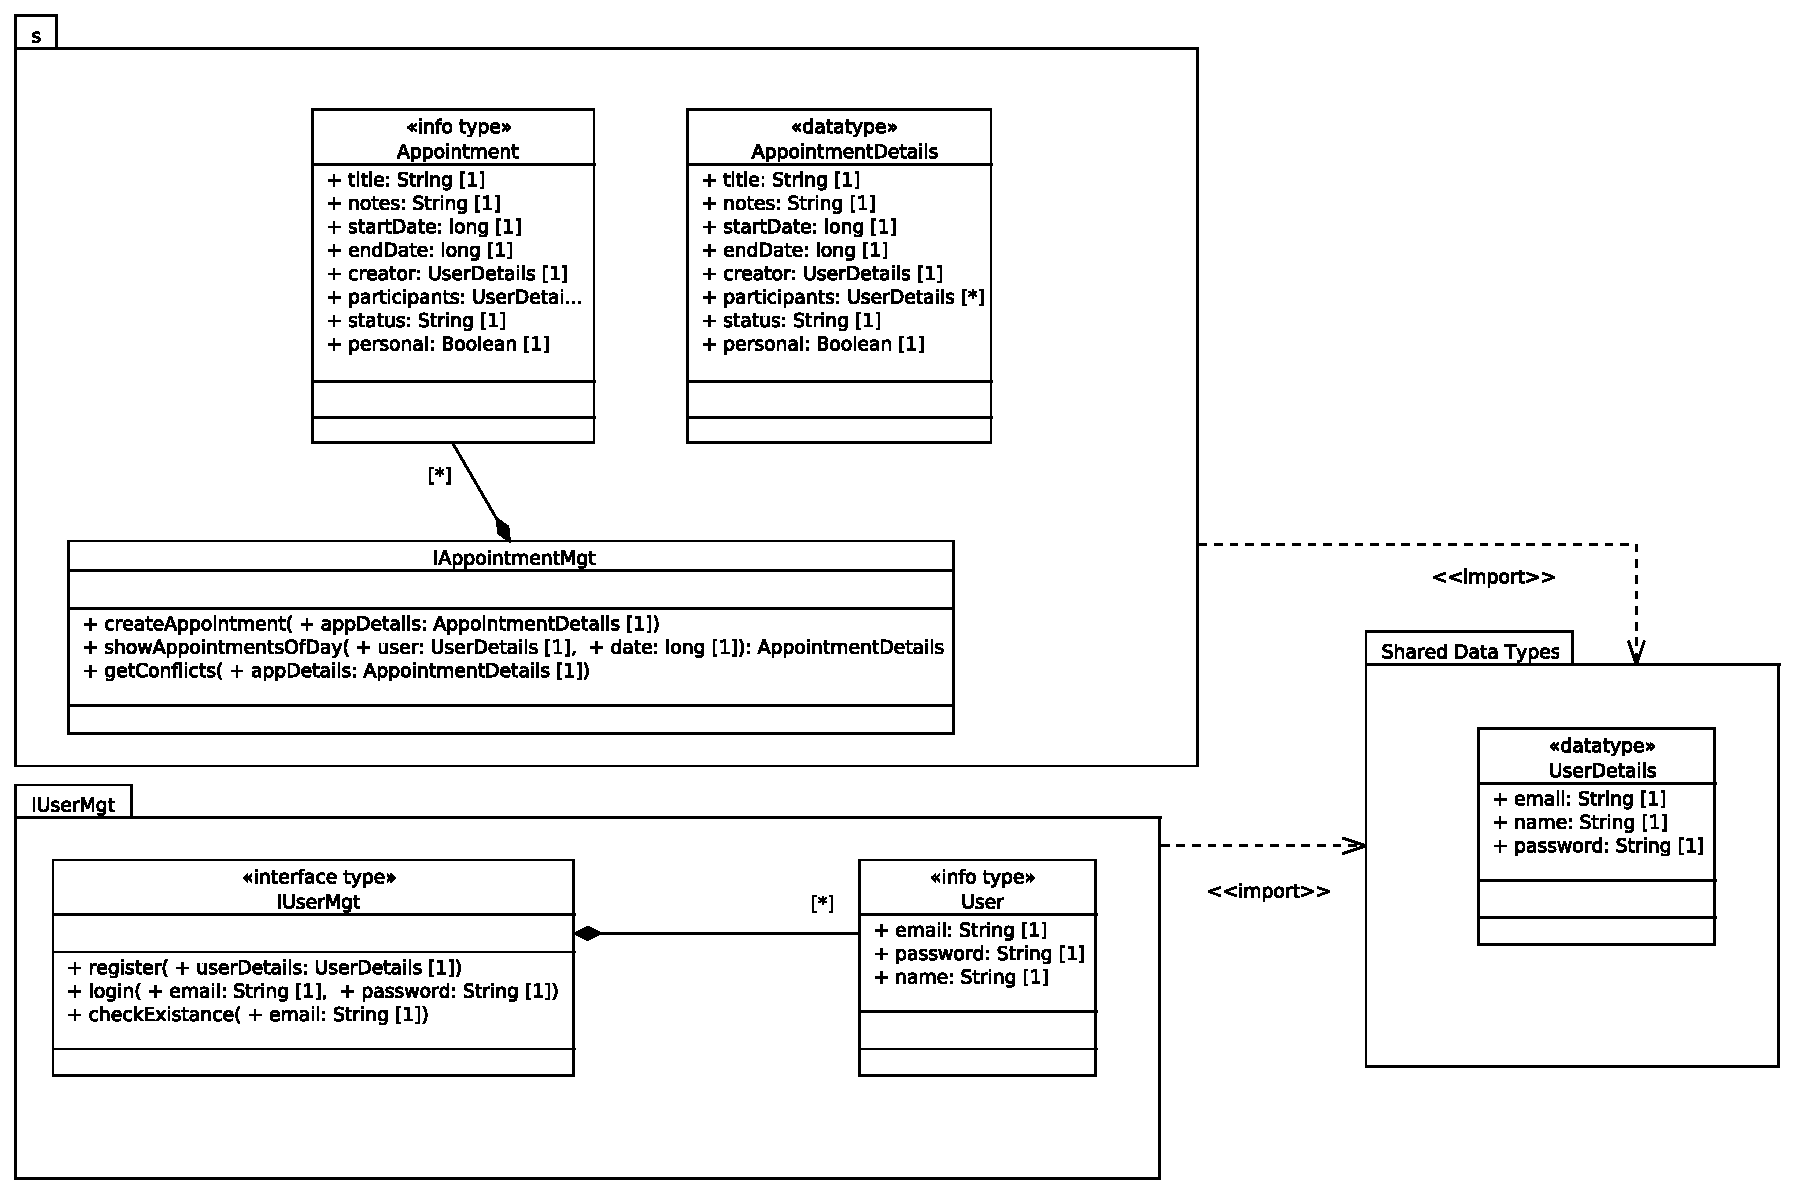
\includegraphics{pictures/InterfaceSpecification}

\end{document}

